\documentclass[]{article}
\usepackage[utf8]{inputenc}
\usepackage[portuguese]{babel}
\usepackage[a4paper]{geometry}
\usepackage{tikz}

\newcommand{\newlog}[2]{%
  \par
  \vspace{\baselineskip}
  \noindent
  #1\\
  \textbf{#2}\\
}

\usepackage{icomma, amsmath}


\begin{document}


\newlog{2024-10-08}{Sobre a magnitude de Io}
As imersões e emersões de Io são, é claro, acompanhadas de grande variação da
sua magnitude. Como ao certo se comporta?
Na emersão do dia próximo dia 9, que segundo o Stellarium se iniciará às 3:36:40
(hora de verão, UTC+01:00) a magnitude de Io começa com o valor 5.50 e final
18.50, às 3:40:23. A duração da emersão é assim 3'43''.

As emersões duram sempre o mesmo? A magnitude de Io permanece constante entre
no intervalo entre eventos? A emersão seguinte inicia-se no dia 2024-10-10 às
22:05:13 com magnitude 5.49 e termina às 22:08:56, com magnitude 18.49. A
duração é a mesma. É de esperar uma diminuição das duas magnitudes extremas em
emersões posteriores porque nesta fase a Terra está a aproximar-se de do sistema
joviano. Na última emersão antes da oposição de Júpiter (no dia 6 de Dezembro,
pelas 12:19 UTC), as magnitudes extremas de Io são 4.92 e 17.92s

\newlog{2024-10-13}{Intensidade do efeito de R{\o}mer}
O efeito observado por R{\o}mer é mais pronunciado quando é máxima a velocidade
radial relativa de Júpiter, ou seja, quando se encontra em quadratura. As
póximas quadraturas vão dar-se a 2025-03-02T18:13:13,5 (em afastamento, notam-se
as emersões) e a 2025-10-17T5:30:31 (em aproximação, notam-se as
imersões). Deve ser em torno dessas ocasiões que o efeito é mais perceptível.
Para referência, a oposição de júpiter ocorre em 2024-12-07T20:51:23 e a
conjunção a 2025-06-24T15:20:55:
\begin{center}
  \begin{minipage}{0.65\linewidth}
  \begin{tabular}{lcc}
    \hline
    Oposição                  & 2024-12-07 & 20:51:00\\
    Quadratura de afastamento & 2025-03-02 & 18:13:13\\
    Conjunção                 & 2025-06-24 & 15:20:30\\
    Quadratura de aproximação & 2025-10-17 & 05:30:31\\
    Oposição seguinte         & 2026-01-10 & 08:12:31\\
    \hline
  \end{tabular}\\
{\sf\small (Todas as horas indicadas em UTC.)}
  \end{minipage}
  \hspace{1em}
  \raisebox{-0.5\height}{%
  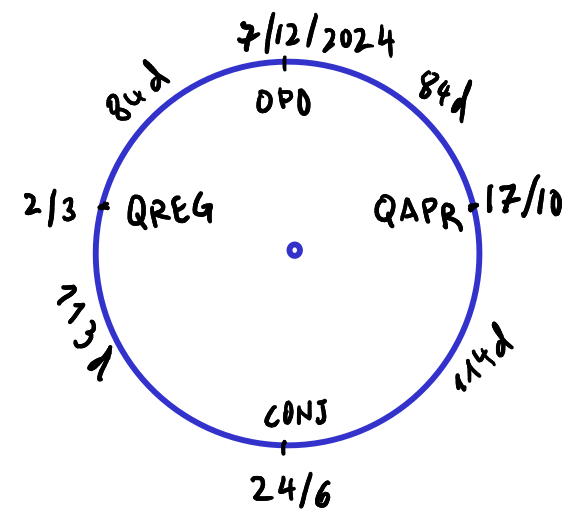
\includegraphics[width=0.25\linewidth]{figs/2024-10-28.png}}\\
\end{center}

\newlog{2024-10-22}{O período das emersões de Io}
Registei as curvas de magnitude das emersões de Io para o período que me foi
atribuído, próximo da quadratura de afastamento no ano de 2025.  Determinei os
momentos das magnitudes médias de cada uma, e as distâncias a que Júpiter se
encontrava nesses instantes. A duração dos intervalos entre emersões sucessivas
apresenta uma oscilação perturbadora, que ilustro no gráfico em baixo:
\begin{center}
  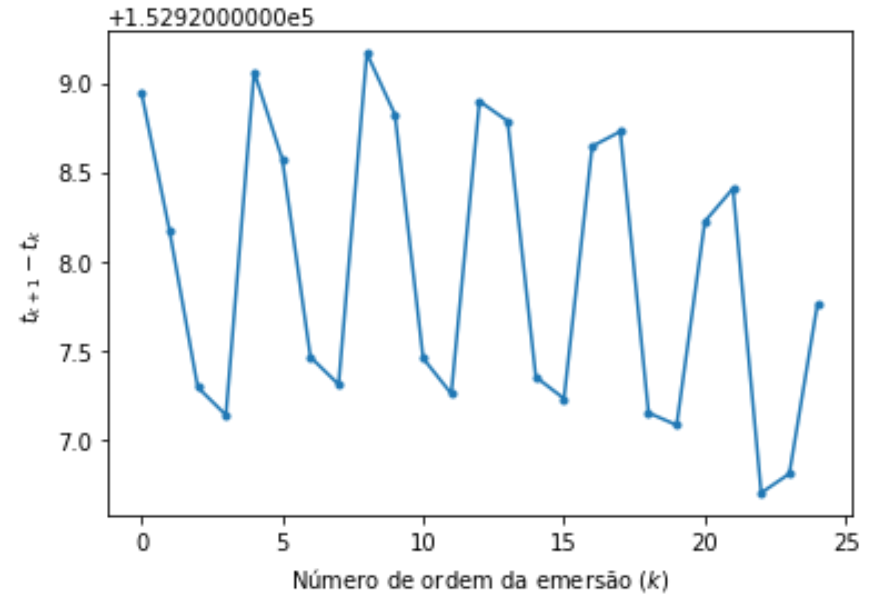
\includegraphics[width=0.5\linewidth]{figs/2024-10-22_a.png}
\end{center}
Note-se que estas oscilações têm uma amplitude aproximadamente 1\,s, em
valores de cerca de $152928\,\text{s}\simeq1,77$\,d. Trata-se, assim de pequenas
oscilações, mas que são comparáveis às que são de esperar devido à variação da
distância Terra Júpiter, que se pretendem usar no cálculo.

A que se pode dever esta oscilação?
\begin{enumerate}
  \item
    Erros de arredondamento do Stellarium por representação discreta do tempo?
  \item
    Estará relacionado com a inconsistência que detetei nos valor apresentado da
    magnitude de Io quando se define a data e hora no script e quando se usa a
    janela de data e hora?
  \item
    Será corrigida fazendo uma interpolação de ordem maior que a linear que
    usei na estimativa do momento da emersão?
  \item
    Ou resulta de algum erro no processo de interpolação usado?
\end{enumerate}

\noindent
Sobre a possibilidade 1:\\
de facto, o Stellarium tem uma representação do tempo mais precisa do que aquela
a que o comando \texttt{core.getDate} permite; este só fornece informação até
aos segundos inteiros, mas é possível, com o comando \texttt{core.setDate}
acertar a hora de forma mais precisa. Isto é relevante? Talvez, uma vez que a
oscilação pode estar relacionada com erros de arredondamento. Vale a pena tentar
reformular o script de geração das curvas de magnitude de forma a aumentar a sua
resolução temporal. O que há a fazer aqui é gerar por software os instantes da
amostragem, com intervalos de meio segundo ou menores, e colocar no output não o
resultado de \texttt{core.getDate} mas uma representação string de cada
instante.

\noindent
Sobre a possibilidade 2:\\
talvez não haja inconsitência nenhuma, talvez essa ideia seja apenas uma
manifestação da o Stellarium ter uma maior resolução temporal do que a da janela
de data e hora.

\noindent
Sobre as possibilidades 3 e 4:\\
Acabo de usar outro esquema de interpolação aplicando a função
\texttt{Akima1DInterpolator} da \textsl{package} \texttt{scipy.interpolate}. Os resultados são
idênticos aos obtidos com a interpolação linear, o que mostra que a oscilação
não resulta do procedimento de interpolação e não apoia a hipótese de haver
erros graves no cálculo. Experimentei outras variantes, sempre com o mesmo
resultado.


\newlog{2024-10-26}{Ainda as oscilações no intervalo entre emersões de Io}
Substituí o método de interpolação linear antes usado por um interpolador por
splines na biblioteca scipy.interpolate (\texttt{InterpolatedUnivariateSpline}).
Os resultados diferem dos anteriormente obtidos apenas nas décimas de milésimas
do segundo. Não parece ser a interpolação a causadora da oscilação. 

\newlog{2024-10-29}{Períodos de tempo a considerar}
Resolvi tomar em conta o período que se inicia 15~dias depois da oposição de
Júpiter de 2024 (a 7 de dezembro) e que termina 15~dias antes da conjugação (a
26 de junho) para as emersões de Io. Este intervalo tem a duração de 168 dias.
Para as imersões, consideraremos um período com a mesma duração (168~dias)
incindo-se igualmente 15~dias depois da conjunção, ou seja, a 9 de julho,
terminando a 24 de dezembro.

\pagebreak[4]
\newlog{2024-11-18}{Atualização ao trabalho desde a entrada anterior}
\nopagebreak[4]
\begin{itemize}
  \item Obtive curvas de magnitude para 43 imersões e emersões centradas nas
    quadraturas
  \item Calculei por regressão linear o valor da velocidade da luz. Os
    resultados não são muito entusiasmantes. Obtém-se cerca de
    $4\times10^8$\,m/s.
  \item
    Reorganizei (e re-reorganizei) os ficheiros. Não sei se já
    acabou essa reorganização. Os ficheiros com as curvas de magnitude estão
    agora em diretorias com nomes \texttt{magc/emergences} e
    \texttt{magc/occultations}, para usar os termos corretos em inglês.
  \item
    Reprogramei o módulo de funções utilitárias, agora com o nome
    \texttt{romer\_utils}. Acho que ficou mais simples e mais prático.
  \item
    Em simultâneo com todas estas reorganizações, fiz várias estimativas de $c$.
    Numa, em particular, fiz um gráfico dos valores de $\Delta d$ vs $\Delta t$,
    para intervalos com diferentes números revoluções de Io (de 1 a 39, todos os
    intervalos centrados nas quadraturas) e calculei $c$ como o declive da reta
    de ajuste. Os resultados não foram espetaculares: $c=3,99\times10^8$\,m/s!
    \begin{center}
      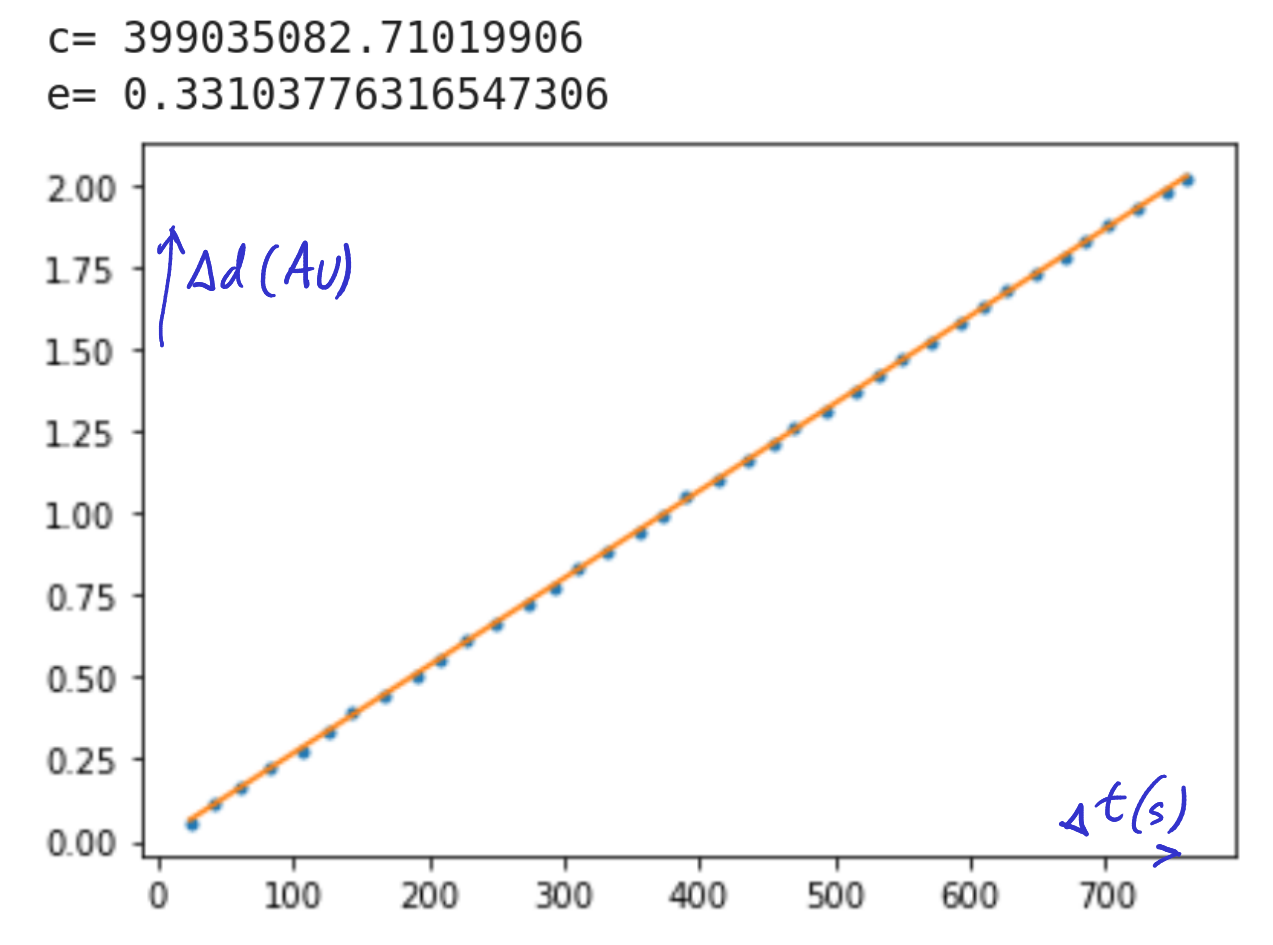
\includegraphics[width=0.5\linewidth]{figs/2024-11-18_a.png}
    \end{center}
    É preocupante o alinhamento dos pontos, indica que não é uma questão de
    precisão. Para cada um destes intervalos, calculei estimativas
    de $c$ independentes e o erro de cada uma, que está representado no gráfico
    em baixo (no eixo horizontal está representado o número de revoluções do
    intervalo usado).
    \begin{center}
      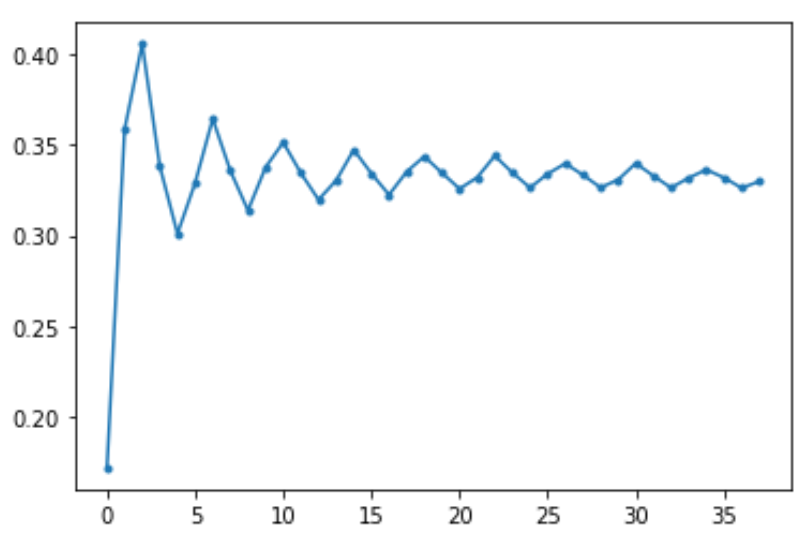
\includegraphics[width=0.5\linewidth]{figs/2024-11-18_b.png}
    \end{center}
\end{itemize}

\newlog{2024-11-24}{Qual o erro de usar a distância instantânea a Júpiter?}
A fórmula que usamos para fazer uma estimativa do valor da velocidade da luz
pelo método de Romer é, considerando $n$ revoluções de Io (logo, $n+1$ emersões
e outras tantas ocultações) é
\begin{equation*}
  c\simeq\frac{(d^{(r)}_n-d^{(r)}_0)-(d^{(a)}_n-d^{(a)}_0)}%
  {(t^{(r)}_n-t^{(r)}_0)-(t^{(a)}_n-t^{(a)}_0)},
\end{equation*}
onde os sobrescritos $(r)$ e $(a)$ indicam respetivamente variáveis relativas à
fase de regressão, em que a Terra se afasta de Júpiter e são observadas emersões
de Io, e de aproximação, em que se observam ocultações; os subescritos $0$ e $n$
indicam a primeira (ou 0-ésima) e a última emersão ou ocultação.

As distâncias $d^{(x)}_k$ que aparecem nesta fórmula são, em rigor, as
distâncias entre a posição de Io \emph{no momento em que se dá} a emersão ou
ocultação e a da Terra \emph{no momento em que se dá} a observação do evento.
Não é trivial obter do stellarium informação sobre distâncias não instantâneas
como esta; por isso, fazemos a aproximação de usar a distância instantânea entre
a Terra e Io no momento da observação da emersão ou ocultação. Mas mais; uma vez
que a distância Júpiter-Io (cerca de $2,819\times10^{-3}$\,au) é muito menor que
a distância Terra-Júpiter (varia entre 6,22\,au na conjunção e 4,22\,au na
oposição), esta deve ser muito aproximadamente igual à a distância Terra-Io, o
que sugere usar a distância a Júpiter em vez da distância a Io, que é o que
temos estado a fazer.

Qual a importância dos erros envolvidos nestas aproximações? Para tentar ter uma
ideia da resposta a esta questão, programei um modelo simples do sistema
Terra-Júpiter-Io. O modelo é, também uma aproximação: considera que as órbitas
da Terra e de Io são circulares, coplanares e percorridas uniformemente. Usando
os valores médios dos raios das órbitas dos três corpos, os períodos orbitais
da Terra e de Io e ainda o raio de Júpiter, simulei um período sinódico de
Júpiter (entre duas conjunções sucessivas, cerca de 400 dias), e registei os
momentos de todas as emersões e ocultações de Io na sombra de Júpiter,
juntamente com a distância entre a Terra no momento da observação da emersão ou
ocultação e Io no momento da ocorrência em causa, a distância Terra-Io no
momento da observação e a distância Terra-Júpiter no momento da observação.
Considerando os intervalos entre a 10ª e a 103ª emersões e ocultações os valores
que se obtêm são:
\begin{center}
  \begin{tabular}{l|c|c}
    \hline
    Método & estimativa & erro relativo\\
    \hline
    Distância evento-observação  & $2,99792456\times10^8$\,m/s
                                        & $7\times10^{-9}$\\
    Distância síncrona a Io      & $2,99790920\times10^8$\,m/s
                                        & $5\times10^{-6}$\\
    Distância síncrona a Júpiter & $2,99789694\times10^8$\,m/s
                                        & $9\times10^{-6}$\\
    \hline
  \end{tabular}
\end{center}
O erro cometido com qualquer das aproximações (distância a Io ou distância a
Júpiter, em vez de distância desde a emersão ou ocultação até ao ponto onde é
observado) é, de facto, pequeno, inferior a uma milésima de porcento.

\noindent
O programa que gera os dados das emersões e ocultações é
\texttt{progs/errors/errestim.py}.

\newlog{2024-12-02}{Atualização}
Já completámos a lista das ocultações e emersões de Io no próximo ano sinódico
de Júpiter. O problema com o cálculo do módulo da velocidade da luz persiste.

\begin{center}
  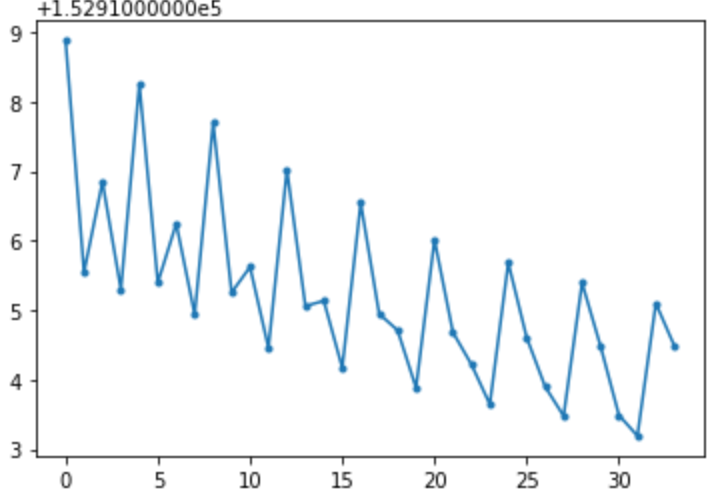
\includegraphics{figs/2024-12-02.png}
\end{center}
Calculei algumas emersões de Io com a opção de simular a velocidade da luz
desativada no Stellarium. A motivação para este esforço foi a suposição de que
desativar esta opção anularia cálculo do atraso com que a luz chega à Terra,
como se a propagação da luz fosse instantânea. Não parece ser o caso (ver a
figura acima).

Experimentei também determinar o momento do início da ocultação de Io ocorrida
hoje pelas 23:22, observada a partir da Terra e de Júpiter. Júpiter encontra-se
a 612,040\,Mkm da Terra, e o início da ocultação é observado em Júpiter 34'20"{}
mais cedo que na Terra. A velocidade da luz resultante é
$2,9792\times10^8$\,m/s, valor muito mais exato do que os que temos obtido.

\newlog{2024-12-03}{Outras possibilidades para estimar $c$}
Hoje estou a tentar outra coisa. O intervalo de tempo entre duas emersões ou
duas ocultações é dado por
\begin{equation*}
  t_n-t_0=nT^*+\frac{d_n-d_0}{c},
\end{equation*}
que podemos reescrever como
\begin{align*}
  \frac{t_n-t_0}{n}&=T^*+\frac{1}{c}\frac{d_n-d_0}{n}.
\end{align*}
A figura em baixo apresenta os valores da duração média entre ocorrências,
$(t_n-t_0)/n$, como função da variação média da distância a Júpiter por
revolução de Io, $(d_n-d_0)/n$.
\begin{center}
  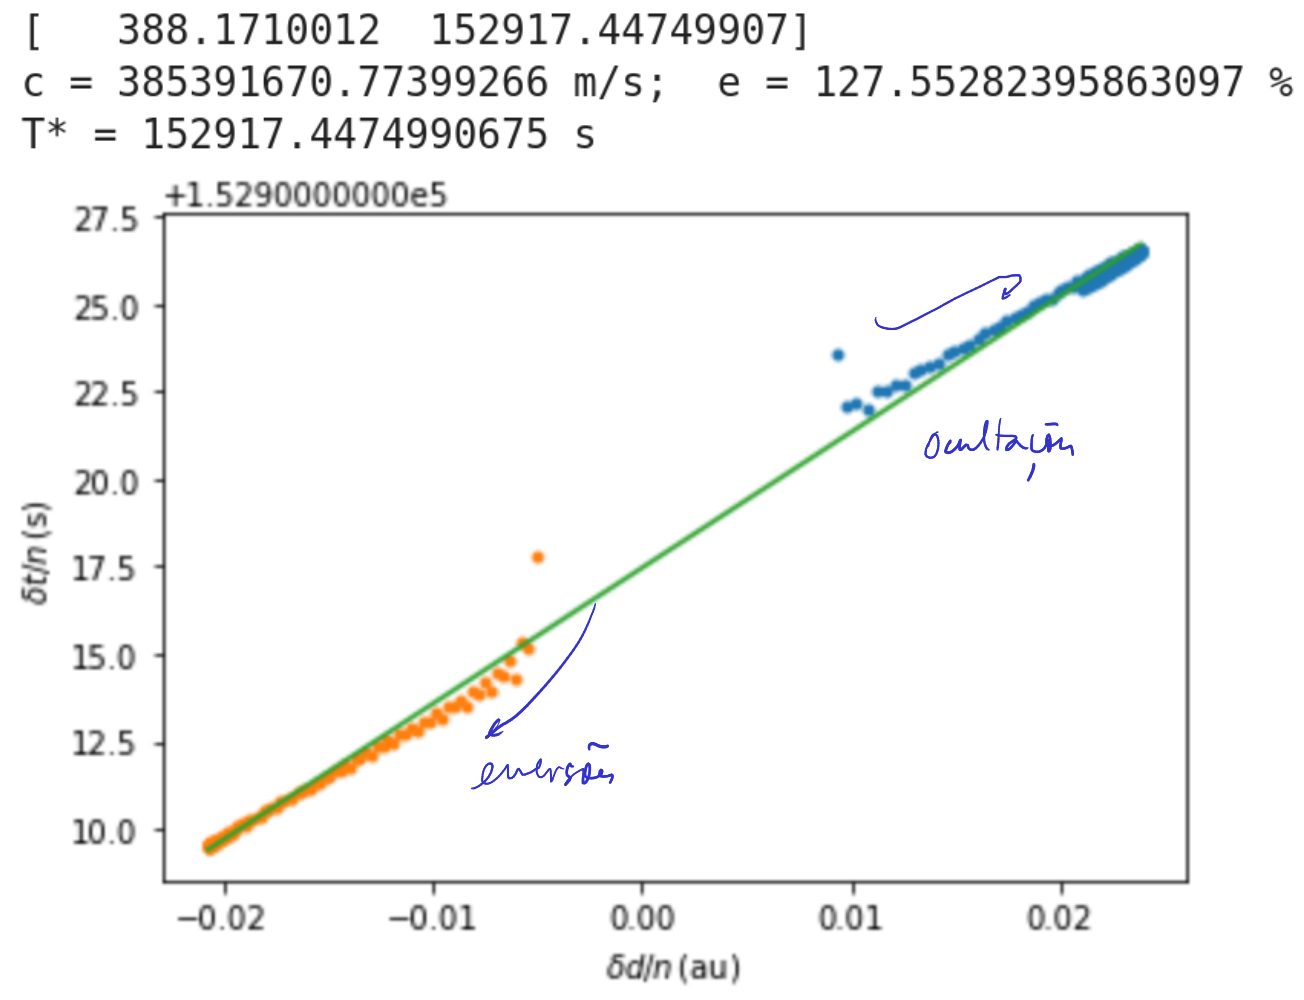
\includegraphics[width=0.6\linewidth]{figs/2024-12-03.png}
\end{center}
O gráfico apresenta também, a verde, a reta de ajuste ao conjunto dos valores.
Os resultados do cálculo são razoáveis para o período orbital de Io, cujo erro
(relativamente ao período sidereal) é de apenas 0,04\%, mas grosseiramente
inexatos relativamente ao declive, que determina o valor da estimativa de $c$.

Note-se que o valor obtido não é tão mau porque os dois grupos de eventos não
estão perfeitamente alinhados. Retas de ajuste a cada um dos grupos teriam
declive menor, o que resultaria a estimativas de $c$ ainda maiores.

Experimentei ainda outra coisa. O stellarium permite simular o céu visto de
outros planetas. Simulei a observação da ocultação de Io de 2024-12-04 a partir
da Terra, de Júpiter e de Io. Os dados foram os apresentados na tabela abaixo.
\begin{center}
  \begin{minipage}[c]{0.4\linewidth}
    \begin{tabular}{l|c}
      \hline
      Local& Hora\\
      \hline
      Terra   & 17:50:21\\
      Io&       17:17:48\\
      Júpiter & 17:16:12\\
      \hline
    \end{tabular}
  \end{minipage}
  \begin{minipage}[c]{0.4\linewidth}
    \begin{align*}
      \overline{TI}&=6,12243\times10^{11}\,\text{m}\\
      \overline{TJ}&=6,11829\times10^{11}\,\text{m}
    \end{align*}
  \end{minipage}
\end{center}
O eclipse é observado na Terra 32'33'' antes que em Io;\footnote{Mas deve ser
  dito que o momento em que o disco de Júpiter e do Sol, vistos de Io, se tocam,
  que usei como marca do eclipse observado de Io, não é o momento em que o disco
  de Io começa a mergulhar na sombra de Júpiter.  O segundo é anterior ao
primeiro.} dada a distância Terra-Io, esta diferença corresponde a
$c\simeq3,135\times10^8$\,m/s. Este valor é ligeiramente alto de mais, em parte
talvez devido à diferença entre os momentos usados para cronometrar o início do
eclipse visto da Terra e de Io. 
Considerando antes a diferença temporal entre as
observações do eclipse da Terra e Júpiter,\footnote{Aqui não se aplica a
chamada de atenção da nota de rodapé anterior.} obtém-se
$c\simeq3,002\times10^8$\,m/s, mais próximo do valor correto.
 
\newlog{2024-12-04}{Métodos para estimar a velocidade da luz}
Considerei até agora três métodos diferentes de estimar $c$ usando as emersões e
ocultações de Io. Para documentar a coisa, vou descrevê-los aqui.

Todos os estes métodos consideram duas (ou um par de duas) emersões ou duas
ocultações de Io que são observadas em instantes $t_0$ e $t_n$ mas que ocorrem
em instantes anteriores $t^*_0$ e $t^*_n$. As duas ocorrências não têm que ser
consecutivas; pelo contrário, considera-se que no intervalo entre elas Io
completa $n$ revoluções em torno de Júpiter (e daí o indice $n$ em $T_n$ e
$t^*_n$). A relação entre os tempos de ocorrência e de observação é, obviamente,
\begin{equation*}
  t=t^*+\delta t_l,
\end{equation*}
onde $\delta t_l=d/c$ representa o tempo do trajeto da luz entre o ponto da
ocorrência e o da sua observação, com comprimento $d$ e percorrido, claro, com
velocidade igual a $c$.\footnote{Como foi discutido no apontamento de 2024-11-24, em vez
desta distância, usamos a distância Terra-Júpiter no instante da observação,
aproximadamente igual.}
Assim, mais explicitamente temos
\begin{align*}
  t_0&=t^*_0+\frac{d_0}{c}& t_n&=t^*_n+\frac{d_n}{c}
\end{align*}
Subtraindo estas duas expressões e tendo em conta que entre as duas ocorrências
Io completa $n$ órbitas com período $T^*$, resulta
\begin{equation}\label{eq:a}
  t_n-t_0=nT^*+\frac{d_n-d_0}{c}.
\end{equation}
Esta expressão é usada nos três métodos apresentados a seguir.


\begin{enumerate}
  \item \textbf{Método simples}\\
    Podemos eliminar o período $T^*$ de revolução na eq.~\eqref{eq:a}
    considerando dois pares de ocorrên\-cias (tendo o cuidado de que o número de
    revoluções completadas por Io seja o mesmo em ambas) e subtraindo as
    expressões correspondentes membro a membro. Resulta
    \begin{equation}\label{eq:b}
      c\simeq\frac{(d_n-d_0)-(d'_n-d'_0)}{(t_n-t_0)-(t'_n-t'_0)}.
    \end{equation}
    O método apresentado por R{\o}mer é essencialmente um caso particular deste,
    tomando como um dos intervalos o período entre a oposição de Júpiter e a sua
    conjunção (ou melhor, entre as duas emersões de Io mais próximas dessas
    situações) e o período entre a conjunção e a oposição seguinte (ou melhor,
    novamente, entre as duas ocultações mais próximas). Resulta
    nesse caso particular
    \begin{equation*}
      c\simeq\frac{4\text{AU}}{(t_n-t_0)-(t'_n-t'_0)}.
    \end{equation*}
  \item \textbf{Regressão linear com quartetos}\\
    Podemos reescrever a eq.~\eqref{eq:b} na forma
    \begin{equation*}
      \left\{(\strut t_n-t_0)-(t'_n-t'_0)\right\}\simeq\frac{1}{c}
      \left\{(d_n-d_0)-(d'_n-d'_0)\strut\right\}
    \end{equation*}
    Num gráfico em que se representem os valores do termo entre chavetas no
    primeiro membro nas ordenadas e os do termo entre chavetas no segundo nas
    abcissas, a reta que melhor se ajusta aos pontos representativos dos dados
    deve ter declive igual ao inverso de $c$. No apontamento do dia 2024-11-18
    foram discutidos resultados obtidos com este método.

  \item \textbf{Regressão linear com pares}\\
    Podemos também reescrever a eq.~\eqref{eq:a} como
    \begin{equation}
      \left\{\frac{t_n-t_0}{n}\right\}
        =T^*+\frac{1}{c}\left\{\frac{d_n-d_0}{n}\right\}.
    \end{equation}
    Num gráfico em que se representem os valores do termo entre chavetas no
    primeiro membro nas ordenadas e os do termo entre chavetas no segundo nas
    abcissas, a reta que melhor se ajusta aos pontos representativos dos dados
    deve ter declive igual ao inverso de $c$ e ordenada na origem igual ao
    período orbital de Io. Este método foi usado para obter os resultados
    apresentados no dia 2024-12-03.
\end{enumerate}

\newlog{2024-12-5}{Novo cálculo com o método simples}
Os resultados apresentados na entrada do dia 2024-11-18 foram calculados usando
o método simples, e intervalos centrados nas quadraturas com diferentes
durações. Hoje faz-se um cálculo ligeiramente diferente. Com a duração dos
intervalos fixa, variam-se os eventos iniciais. Os resultados não são
brilhantes. A figura em baixo mostra os valores de $c$ obtidos com intervalos de
diferentes durações (contendo os números de revoluções apresentados na legenda),
correndo ao longo do ano sinódico. As curvas começam na primeira data disponível
nas séries de emersões e de ocultações e vão até à última possível (a que se
encontra a $n$ eventos do final da série).
\begin{center}
  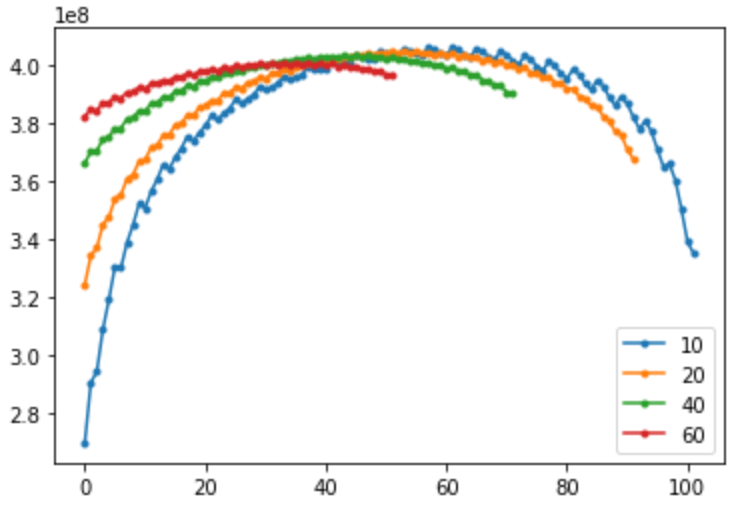
\includegraphics[width=0.5\linewidth]{figs/2024-12-05.png}
\end{center}

Não sei qual possa ser o significado disto, mas quando o número de revoluções
nos intervalos usados é ímpar, nota-se uma oscilação intensa nos valores
resultantes para $c$ em função das alturas em que se situam os intervalos. Por
exemplo, para $n=21$ o resultado é o ilustrado na figura abaixo
\begin{center}
  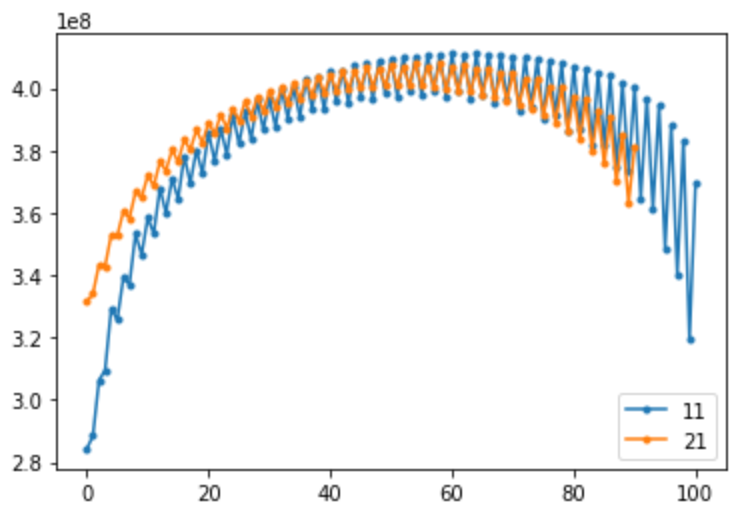
\includegraphics[width=0.5\linewidth]{figs/2024-12-05b.png}
\end{center}

Outra coisa que fiz hoje foi comparar um cálculo com um quarteto de
acontecimentos concreto com o que se obtém substituindo as distâncias a Júpiter
pelas (mais corretas) distâncias a Io. Como suspeitava, os resultados são
idênticos:
\begin{align*}
  c_{TJ}& = 3,99893\times10^8\,\text{m/s}&
  c_{TI}& = 3,99892\times10^8\,\text{m/s}
\end{align*}
\end{document}
